% (The MIT License)
%
% SPDX-FileCopyrightText: Copyright (c) 2023-2025 Yegor Bugayenko
% SPDX-License-Identifier: MIT

\documentclass{article}
\usepackage{../pmba}
\newcommand*\thetitle{Communications Mgmt}
\begin{document}

\lnTitlePage{7}{10}{uUFWVA4We34}

\pmbaQuestion
  {A customer \emph{asks}: ``What's up? How is my project going?'' What do you answer?}
  {Why do you ask?}
  {CPI = 0.85, SPI = 1.12}
  {We are behind the schedule, but under the budget}
  {We are fully committed to deliver on time, as promised!}
  {status-report}

\pmbaQuestion
  {A new programmer joins your team. How do you \emph{explain} her the architecture of the software?}
  {Ler her spend some time in pair programming with a mentor}
  {Show her the code}
  {Schedule a meeting with the entire team}
  {You don't}
  {soft-skills}

\pmbaQuestion
  {On a ``Daily Standup'' meeting, one programmer, when \emph{you ask} him ``What have you done yesterday'' keeps saying ``I don't remember.'' How to fix this?}
  {Fire him}
  {Ask him to be more respectful to the team}
  {Demand written daily reports}
  {Stop asking him}
  {standup}

\pmbaQuestion
  {You see that meetings in your team take too much time, people \emph{waste time} in long and \emph{chaotic} discussions. How do you fix this?}
  {Request meeting agendas}
  {Demand meeting minutes}
  {Appoint meeting facilitator}
  {Reduce amount of meetings}
  {meetings}

\pmbaQuestion
  {After you allowed your team to work \emph{remotely}, the performance of a few programmers dropped significantly. How do you fix this?}
  {Make regular daily Zoom calls with them}
  {Fire them}
  {Pay them more}
  {Ask them to return back to the office}
  {remote-work}

\pmbaQuestion
  {Your programmers are paid on a monthly basis, and you can't change this. The project is \emph{boring} and team performance is very low. What can you do?}
  {Communicate project objectives regularly}
  {Make regular/daily status meetings}
  {Ask everybody to send daily reports}
  {Find a better job}
  {guilt}

\pmbaQuestion
  {A programmer didn't complete his task and explains: ``I misunderstood the ticket description''. This is caused by \emph{low quality} of what?}
  {Communication}
  {Documentation}
  {Requirements}
  {Motivation}
  {responsibility}

\pmbaQuestion
  {You \emph{friend} has been promoted, while you know that his code contribution is smaller than yours and the quality is lower. How can you get even?}
  {You can't; quit the project}
  {Stop considering him a friend}
  {Tell your boss that it's not fair}
  {Move your desk closer to your boss}
  {boss}

\plush{
  \pptBanner{Homework:}
  \begin{multicols}{2}
  ``\emph{Communications Management Plan}'' is a component of a project management plan that describes
  how project communications will be planned, structured, monitored, and controlled. --- PMBOK5
  \par\columnbreak\par
  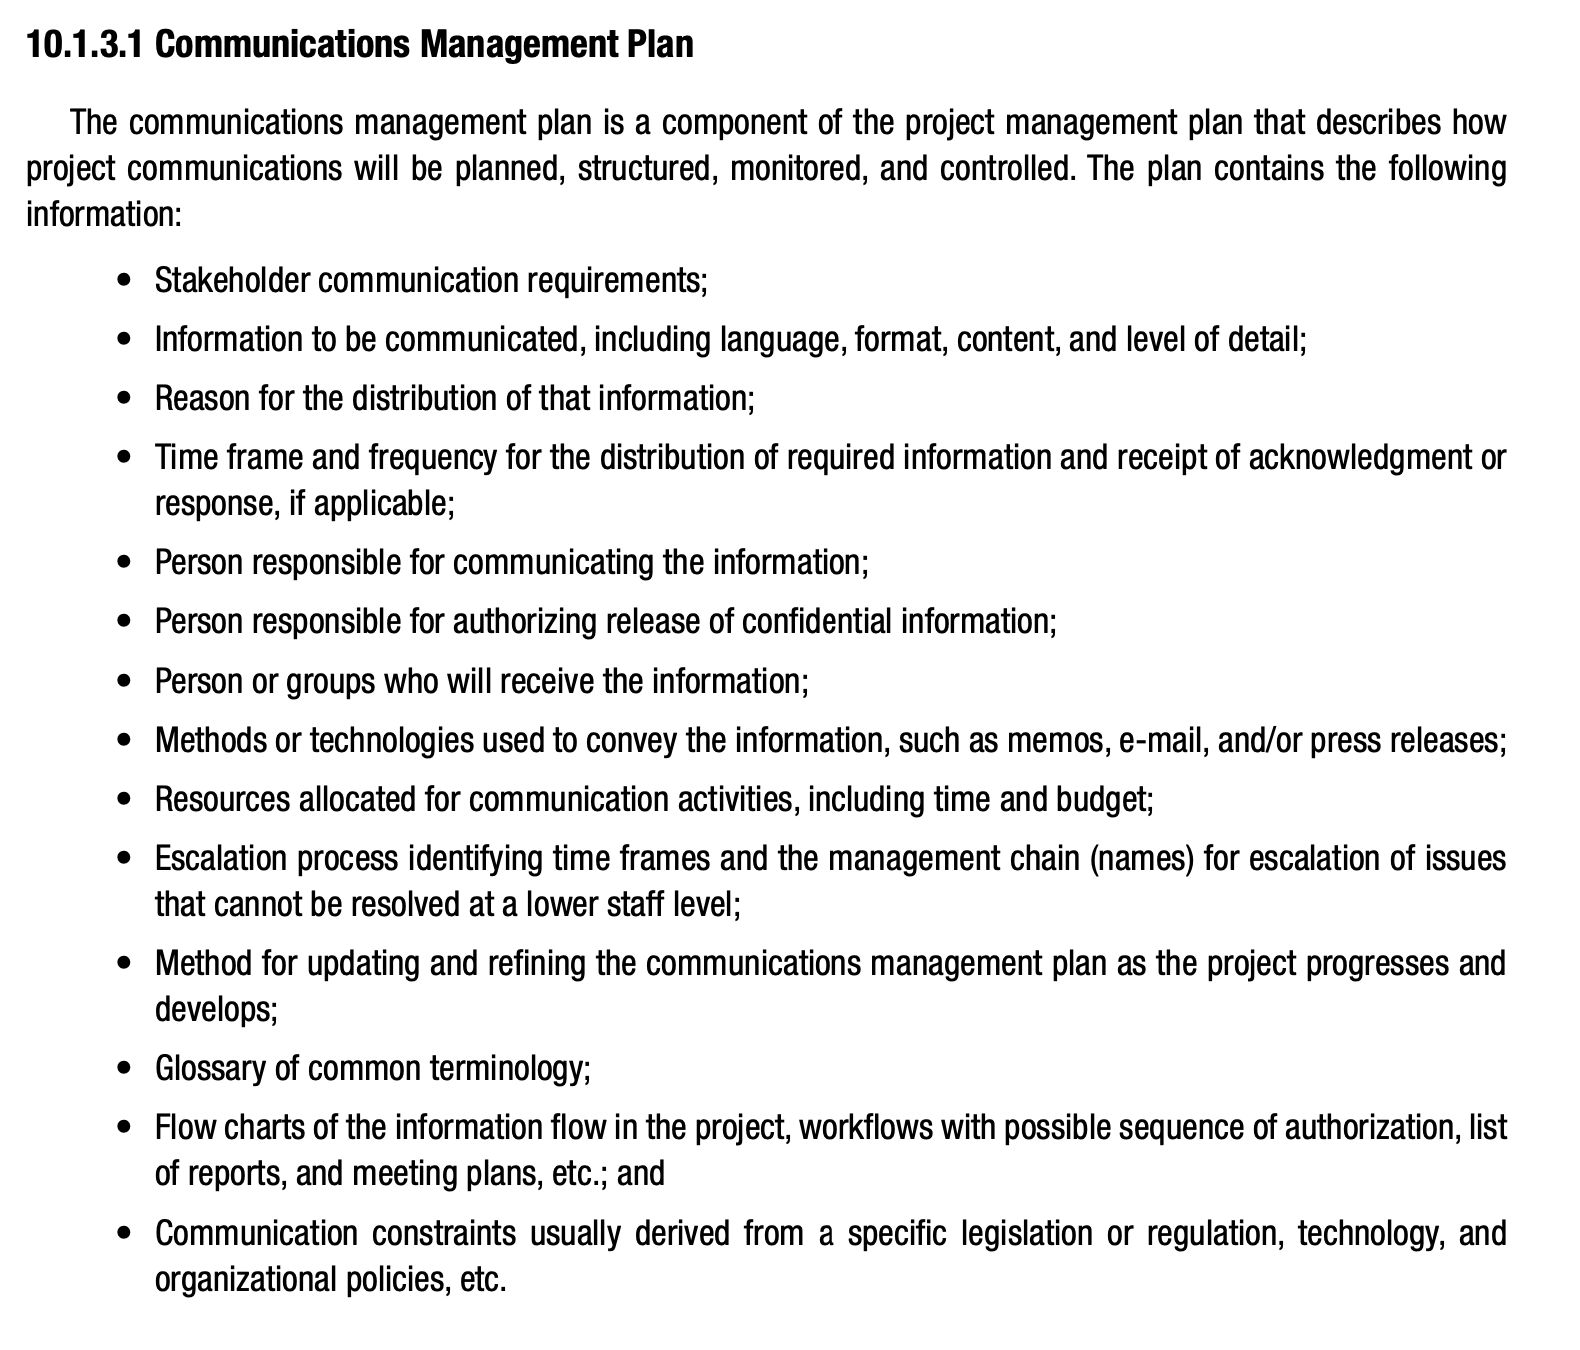
\includegraphics[width=\columnwidth]{plan.png}
  \end{multicols}
}

\plush{
  \pptBanner{Read this:}
  \href{https://www.yegor256.com/2018/08/29/soft-skills.html}{Soft Skills Demystified} (2018)\par
  \href{https://www.yegor256.com/2016/08/23/communication-maturity.html}{Eight Levels of Communication Maturity} (2016)\par
  \href{https://www.yegor256.com/2020/12/29/metric-for-emotions.html}{Put a Number on Your Boss's Emotions} (2020)\par
  \href{https://www.yegor256.com/2020/11/03/daily-reports.html}{The Pain of Daily Reports} (2020)\par
  \href{https://www.yegor256.com/2019/09/03/injection-of-guilt.html}{Daily Stand-up Injection of Guilt} (2019)\par
  \href{https://www.yegor256.com/2016/08/05/distributed-teams-are-higher-quality.html}{A Distributed Team Delivers Code of Higher Quality} (2016)\par
  \href{https://www.yegor256.com/2015/07/13/meetings-are-legalized-robbery.html}{Meetings Are Legalized Robbery} (2015)\par
  \href{https://www.yegor256.com/2015/01/08/morning-standup-meetings.html}{Daily Stand-Up Meetings Are a Good Tool for a Bad Manager} (2015)\par
}

\end{document}
